\section{Evaluation}
\label{cha:evaluation}

We evaluate our design by first implementing it, then running the experiment using it and concluding with analysing the results of the experiment.

\subsection{Implementation}
\label{sec:implementation}

\subsubsection{Dataset Generator}
We have decided to not use an off the shelf dataset or dataset generator like BerlinMOD \cite{duntgenBerlinMODBenchmarkMoving2009}, but to implement our own generator.

We developed a data generator simulating e-scooter trips in Berlin using Python 3.\footnote{\url{github.com/erykksc/escooter-trips-generator}}
We used the OpenStreetMap data through OSMnx library to extract the biking network, points of interest and administrative boundaries (in the rest of the thesis we refer to them as localities).

Inside the repository we also define a flake.nix file, which allows us to match the exact versions of Python interpreter and all the libraries used using nix, ensuring repeatability and reproducibility of the dataset generation.
Additionally we use a seed value in order for the pseudo random generators to yield the same dataset each run.

Using the generator we simulate 1 billion trips from 01-01-2020 to 31-12-2025.
The generator create trips in a following manner:
\begin{enumerate}
  \item Start point and start time of every trip are chosen randomly from uniform distributions seen on \cref{fig:trip-start-point-distribution} and \cref{fig:trip-time-distribution}
  \item A random bearing is chosen, also from a uniform distribution seen on \cref{fig:trip-bearing-distribution}
  \item The route traverses through nodes in a direction of a random bearing, choosing nodes with the smallest bearing difference to our chosen bearing.
    We extend the route by adding nodes to it until we reach the threshold length defined by a Log-normal distribution with $\alpha=0.5$, scale=2100 (median ~2100m) seen on \cref{fig:trip-route-length-distribution}.
  \item We model the speed between the nodes along the trip with a Beta distribution with $\alpha=8, \beta=1$ scaled to 0-20 km/h, seen on \cref{fig:trip-speed-distribution}.
    We chose this distribution as 20km/h is max legal speed in Germany and a driver needs to slow down on turns or traffic lights but tends to ride close to the max speed.
  \item Using the speed and the distance between the nodes, the time to travel between the nodes is computed.
  \item Using the route, start time, and time to travel between individual nodes of the route, we create a single trip.
    A trip consist of many events.
    An event is a single data entry with following fields and types:
    \begin{itemize}
      \item \textbf{event\_id} - UUIDv4
      \item \textbf{trip\_id} - UUIDv4
      \item \textbf{timestamp} - ISO 8601 timestamp with timezone offset
      \item \textbf{latitude} - float
      \item \textbf{longitude} - float
    \end{itemize}
\end{enumerate}

\begin{figure}
  \begin{subfigure}{0.49\linewidth}
    \centering
    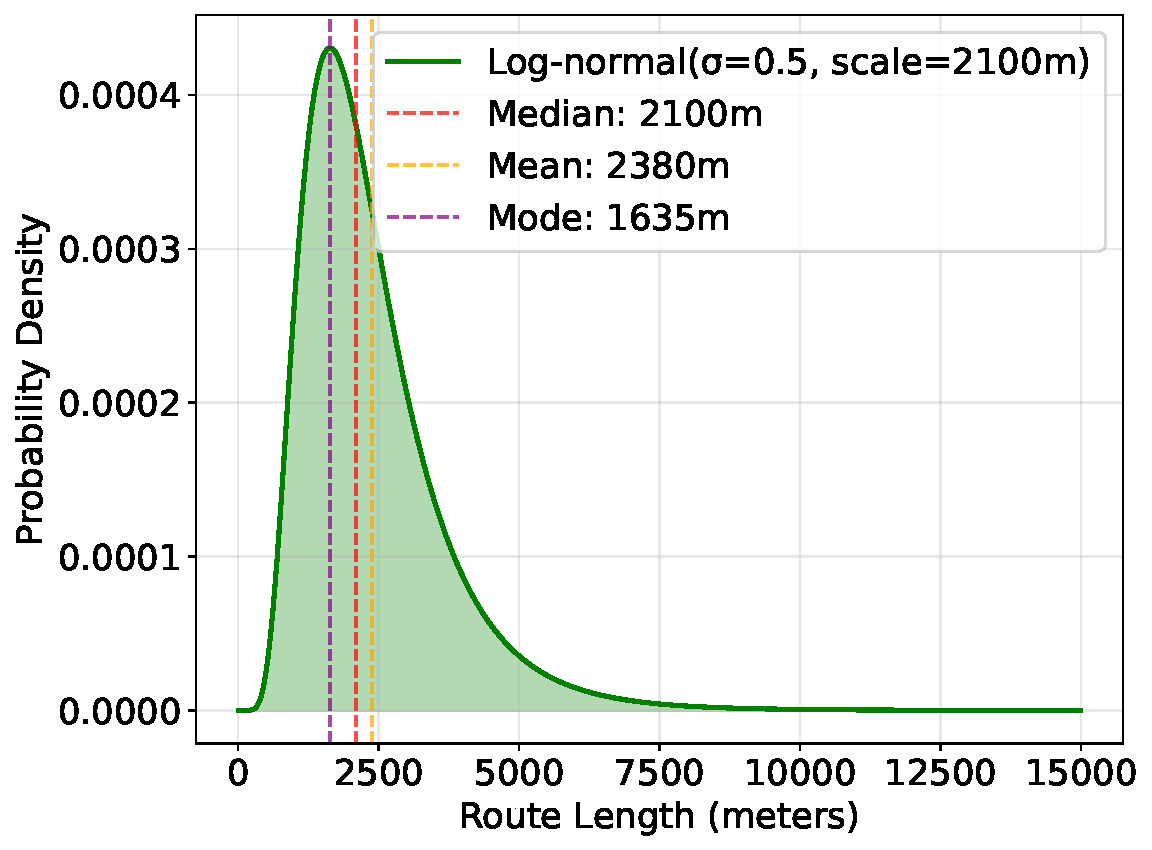
\includegraphics[width=\linewidth]{./fig/route-length-distribution-no-labels.pdf}
    \caption{Route length distribution}
    \label{fig:trip-route-length-distribution}
  \end{subfigure}
  \hfill
  \begin{subfigure}{0.49\linewidth}
    \centering
    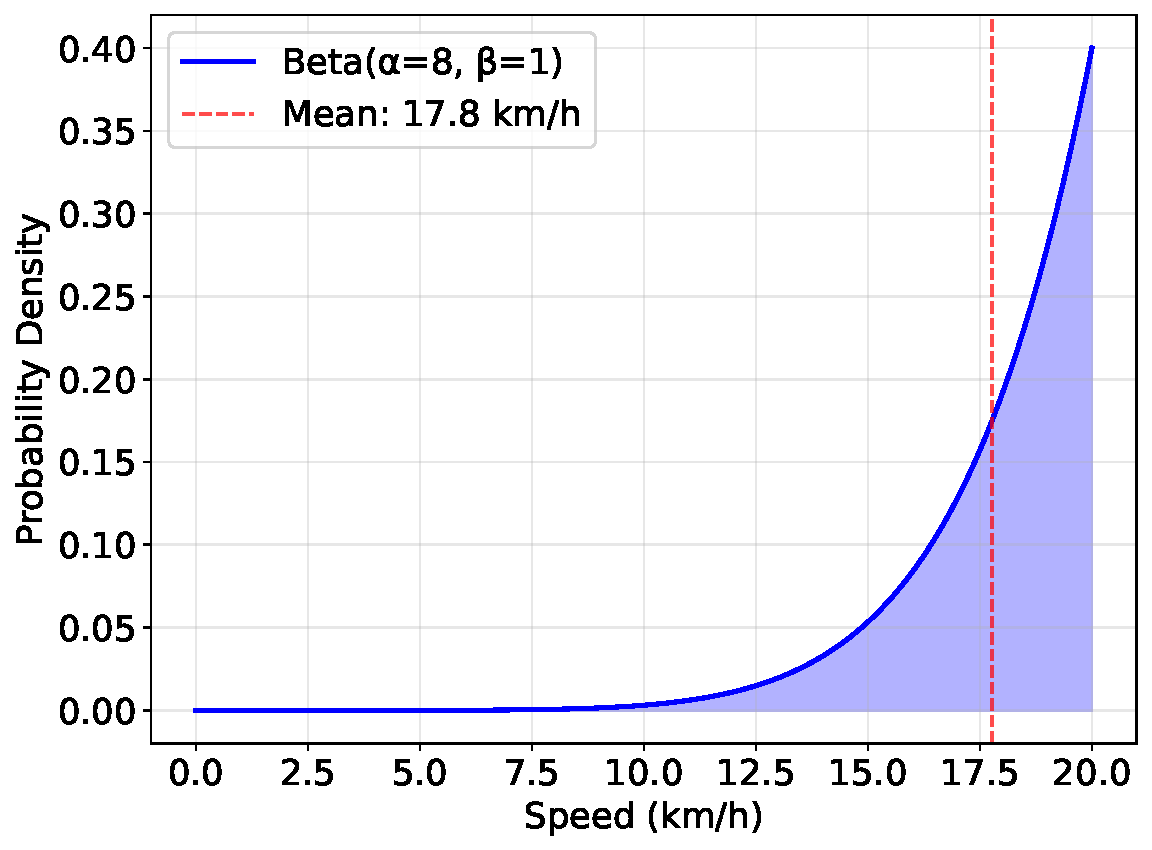
\includegraphics[width=\linewidth]{./fig/speed-distribution-no-labels.pdf}
    \caption{Escooter speed distribution}
    \label{fig:trip-speed-distribution}
  \end{subfigure}
  \vfill
  \begin{subfigure}{0.49\linewidth}
    \centering
    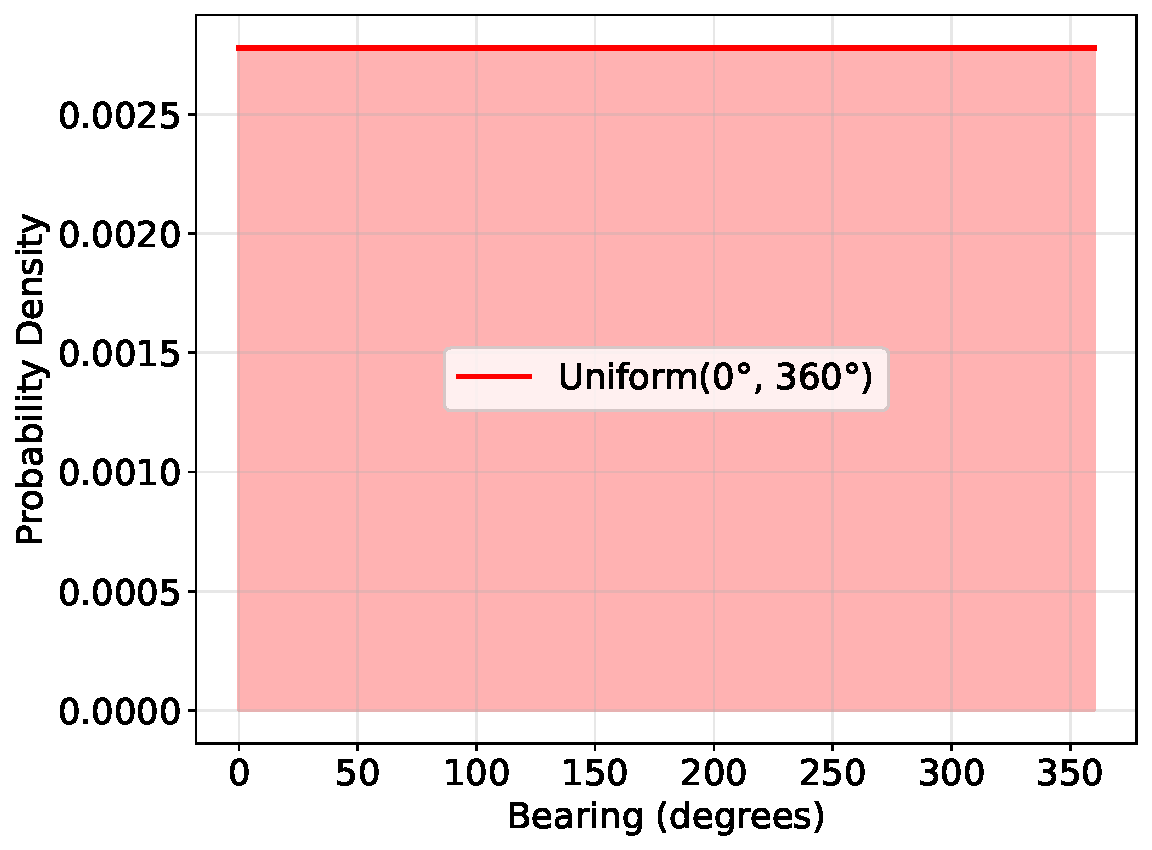
\includegraphics[width=\linewidth]{./fig/bearing-distribution-no-labels.pdf}
    \caption{Bearing of a trip distribution}
    \label{fig:trip-bearing-distribution}
  \end{subfigure}
  \hfill
  \begin{subfigure}{0.49\linewidth}
    \centering
    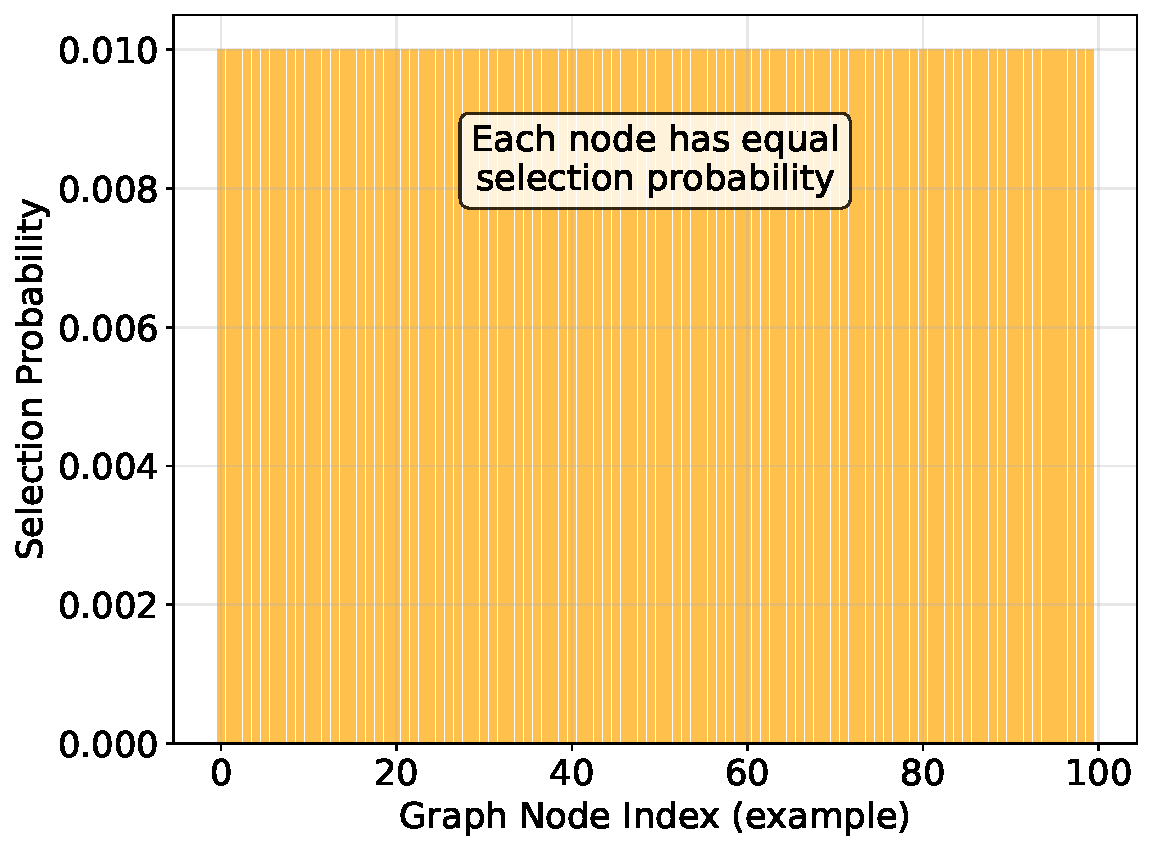
\includegraphics[width=\linewidth]{./fig/start-point-distribution-no-labels.pdf}
    \caption{Start point of a trip distribution}
    \label{fig:trip-start-point-distribution}
  \end{subfigure}
  \vfill
  \begin{subfigure}{0.49\linewidth}
    \centering
    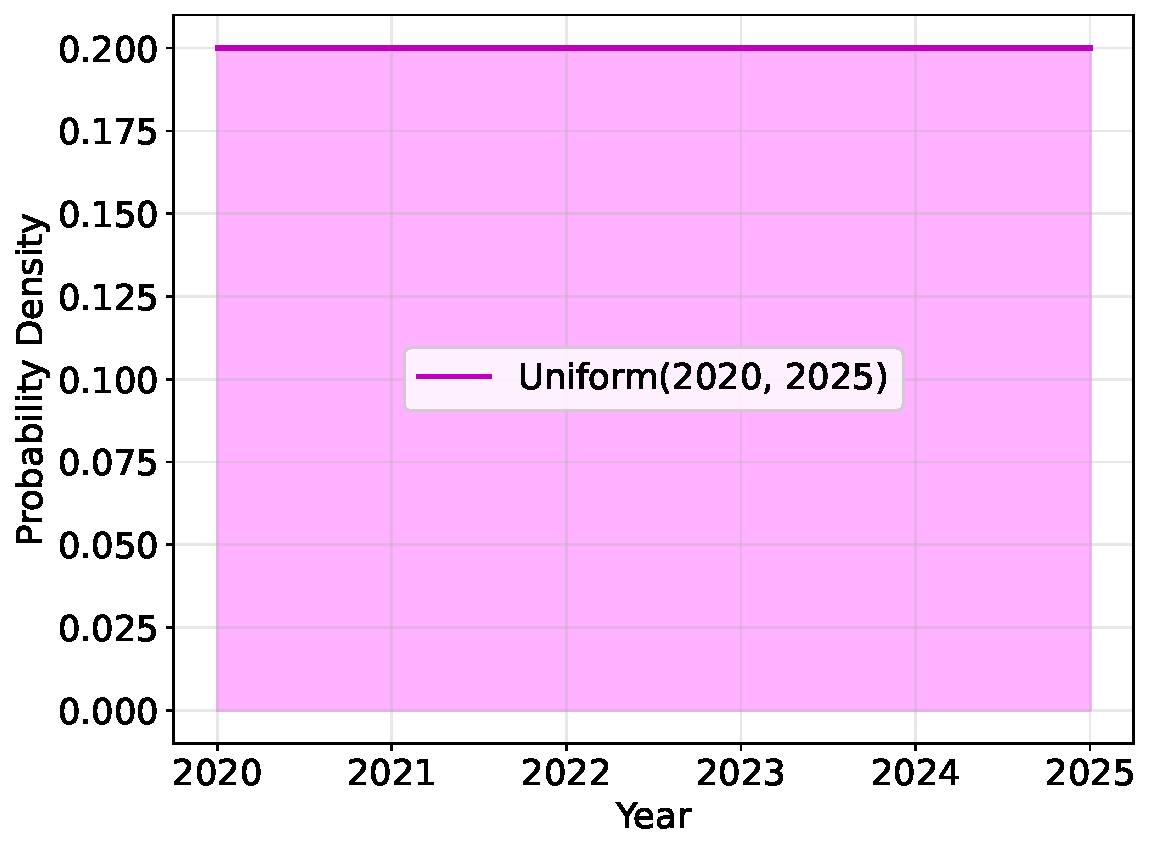
\includegraphics[width=\linewidth]{./fig/time-distribution-no-labels.pdf}
    \caption{Start time of a trip distribution}
    \label{fig:trip-time-distribution}
  \end{subfigure}
  \caption{Distributions we used in our dataset generator for simulating e-scooter trips}
  \label{fig:generator-distributions}
\end{figure}

We saved the simulated trips into a CSV file for our load-generator to consume.

\subsubsection{Load-Generator}
We implement the load-generator in Go (version 1.24).
We choose this programming language due to its builtin concurrency features:
(1) go-routines - lightweight, user-space threads managed by the Go runtime, and
(2) channels - allow safely communication between go-routines.

We made this decision to simulate many simultaneous DDBMS clients, each consuming little memory.
Goroutines are resource-efficient as the Go runtime performs the N:M mapping of goroutines to OS threads.\footnote{\url{https://go.dev/src/runtime/HACKING}}
This way we can scale to thousands or even millions of concurrent clients on a single machine, as each client is primarily I/O-bound.

Next, we implement 3 modes to the load-generator to run the 3 scenarios from the design:
\begin{enumerate}
  \item \textbf{initialize} - initializes tables and indexes
  \item \textbf{insert} - inserts e-scooter events into DDBMS, implementing the insert scenario
  \item \textbf{query} - queries DDBMS using randomized queries from a file with templates.
    We implement two template files for each DDBMS, one containing the simple queries and the second one implementing the complex queries.
\end{enumerate}

\subsubsection{Insert Queries}
We insert the e-scooter events from the generated CSV file into DDBMS using multiple concurrent connections.

The insert process works on a basis of a work queue, a pattern described by Burns and Oppenheimer \cite{196346} i.e., main thread reads data from the CSV file and adds jobs to the queue.
The workers read the jobs containing the events data from the queue and execute insert queries on the DDBMS while collecting metrics.
Our design of the load-generator can be seen on \cref{fig:load-generator-diagram}.

\begin{figure}[ht]
  \centering
  \begin{tikzpicture}[
      box/.style={draw, minimum width=2, minimum height=1cm, align=center},
      smallbox/.style={draw, minimum width=2.5cm, minimum height=1cm, align=center},
      arrow/.style={->, thick},
      node distance=1.5cm and 1.8cm
    ]

    % Dataset and CSV
    \node[box, fill=red!30] (dataset) {DataSet\\Generator};
    \node[smallbox, above=of dataset] (csv) {E-Scooter\\Trips CSV};

    % Main Thread
    \node[smallbox, right=2cm of csv, fill=blue!30] (mainthread) {Main\\Goroutine};

    % Queue as horizontal cylinder
    \node[draw, cylinder, shape border rotate=180, minimum height=1.8cm, minimum width=1cm,
      cylinder uses custom fill, fill=green!30, cylinder body fill=green!30,
    cylinder end fill=green!30, below=1cm of mainthread] (queue) {Work Queue};

    % Workers
    \node[box, fill=blue!30, above right=1cm and 2cm of queue] (worker1) {Worker 1};
    \node[box, fill=blue!30, below=1cm of worker1] (worker2) {Worker 2};
    \node[box, fill=blue!30, below=1cm of worker2] (workerN) {Worker N};

    % Bounding box for LOAD-GENERATOR
    \node[draw, thick, dashed, fit={(mainthread) (worker1) (worker2) (workerN)},
    label=above:LOAD-GENERATOR, inner sep=0.9cm] (loadgen) {};

    % SUT clearly outside the bounding box to the right
    \node[box, right=0.9cm of loadgen, fill=yellow!30] (sut) {SUT};

    % Result Files centered below LOAD-GENERATOR
    \node[box, below=1cm of loadgen.south] (result) {Measurements and Logs};

    % Arrows
    \draw[arrow] (dataset) -- node[right] {generates} (csv);
    \draw[arrow] (mainthread) -- node[above, fill=white] {reads} (csv);
    \draw[arrow] (mainthread) -- node[left, align=center] {inserts\\jobs} (queue);

    \draw[arrow] (queue.east) -- node[align=center, fill=white] {reads\\job} (worker1.west);
    \draw[arrow] (queue.east) -- (worker2.west);
    \draw[arrow] (queue.east) -- (workerN.west);

    \draw[<->, thick] (worker1.east) -- node[fill=white] {queries} (sut);
    \draw[<->, thick] (worker2.east) -- (sut);
    \draw[<->, thick] (workerN.east) -- (sut);

    \draw[arrow] (loadgen.south) -- node[right] {saves results} (result.north);
  \end{tikzpicture}
  \label{fig:load-generator-diagram}
  \caption{}
\end{figure}

The queue is implemented using go-channel avoiding race conditions and manual mutex locks as the go-channels provide built-in synchronization.
Individual worker threads measure the metrics from the DDBMS alongside the time they have spent waiting for their next job (ideally, wait time for next job should be 0).
We have added this mechanism in order to ensure that the speed at which main thread reads from file is not a bottleneck as this would make load-generator a bottleneck in the benchmark.

We implemented two modes of inserts into load-generator: batch and bulk.
In the batch mode we insert multiple single SQL queries into a single request, reducing the network trips.
We made the batch size configurable so it is possible to send single insert queries.
On the other hand, in the bulk we send single request with a configurable amount of events.

\subsubsection{Read Queries}

We split the read queries into two categories, simple and complex.
By doing that we want to simulate two user categories (1) clients (2) analysts.

Consequently, the simple queries, the ones simulating individual clients, consist of queries that query for information about a single trip.
We have identified 8 queries relevant for an e-scooter user:
\begin{enumerate}
  \item \textbf{Length of a trip} - retrieve the length of a specific trip (e.g., in the summary after a trip)
  \item \textbf{Trip events} - retrieve all events of a trip (e.g., in order to display them on a map)
  \item \textbf{Average speed of a trip} - retrieve average speed during the trip (e.g., in the summary after a trip)
  \item \textbf{Trip start locality} - retrieve the locality the trip started in (i.e., part of the city where the trip started)
  \item \textbf{Trip finish locality} - retrieve the locality the trip ended in (i.e., part of the city where the trip ended)
  \item \textbf{First and last location of a trip} - retrieve the first and last location of a trip (e.g., in order to show simplified summary view on a map)
  \item \textbf{POIs close to the finish location} - retrieve points of interest in a specific radius around the finish location (e.g., in order to show shops nearby)
  \item \textbf{POIs within radius during the trip} - retrieve which points of interests the user has driven past through during his trip (e.g., in order to mark certain touristic attractions as visited)
\end{enumerate}

After the simple queries, we define 7 complex queries.
Those queries aim to mimic the queries an analyst may sent to DMBS in order to gain insight into traffic, find possible optimization points.
In order to imitate that we defined the following queries, each of them queries about a specific time frame:
\begin{enumerate}
  \item \textbf{Trips in locality} - Which trips have passed through a specified locality in time frame
  \item \textbf{Most visited POIs} - which points of interests had trips that were in specified distance from them in a specified time frame
  \item \textbf{N closest trips to POI} - find n trips that came the closest to a point of interest in a specified time frame
  \item \textbf{Average trip duration per locality} - calculate the average trip duration per locality in a specified time frame
  \item \textbf{Start and end in different localities} - how many trips started and ended in different locality in a specified time frame
  \item \textbf{Event density heat-map per locality} - generate heat-map of e-scooter usage by area and hour
  \item \textbf{Trips summaries} - summaries about trips in time frame e.g., minimal, maximal, average of length, duration of a trip as well as of the event count for trips
\end{enumerate}

% TODO: add the section that mobilitydb is inspired from the tutorial and then the cratedb has been
% created to mimic this functionality. There were
The queries are inspired by the online tutorial [FOOTNOTE LINK], but have been adapted fo

All the queries are parametrized so they do not repeat.
We generate the actual queries on the fly inside the load-generator during execution.
The random generator is set to a seed and we use a work queue pattern, same as in the insert mode.
As the seed is set based on the query number and base seed, allowing reproducibility of every query.
We choose a query template in a rotating fashion, so that the each subsequent template is different from the past one.
This ensures that we will not be biased towards one DDBMS by generating different queries for it.

\subsubsection{Infrastructure}
We implemented the infrastructure as code using OpenTofu, an open source terraform fork.\footnote{\url{https://opentofu.org/}}
Using it we defined three deployments:
\begin{enumerate}
  \item \textbf{Shared} - defines shared infrastructure between load-generator and AKS-cluster i.e., subnet, virtual network, and a resource group
  \item \textbf{Load-Generator} - defines the virtual machine (VM) used as load-generator
  \item \textbf{AKS Cluster} - defines Kubernetes cluster running on Azure Kubernetes Service (AKS)
\end{enumerate}

Using three deployments allows us to take down the Kubernetes cluster without affecting the load-generator VM.
This is important as the load-generator stays the same between benchmark runs and the size of the AKS-cluster changes.

\subsubsection{DDBMS Deployment}

We have decided to use Docker for containerization of the DDBMS in order to improve portability and allow easy local development.
We automated the deployment by choosing Kubernetes as the container orchestration tool.
We chose it compered to other container orchestration tools like Docker swarm, as it has the widest adoption by developers\footnote{\url{https://survey.stackoverflow.co/2025/technology/\#1-cloud-development}}, thus improving relevancy of the benchmark, as it is more likely that DDBMS will be deployed this way. We used the provided official Kubernetes operator to deploy the CrateDB clusters.

For the MobilityDBC was no official nor unofficial docker image at time of writing, so we developed our own\footnote{\url{https://github.com/erykksc/citus-mobilitydb}}.
Moreover, we published this image to GitHub Container Registry (GHCR) under MIT License.\footnote{\url{ghcr.io/erykksc/citus-k8s-manager:latest}}
We use PostgreSQL 17 image as base for the image as it is the latest supported version by Citus at time of writing.\footnote{\url{https://www.citusdata.com/updates/v13-0/}}
Then, we use the official instructions for Debian from Citus webpage on top of PostgreSQL to install Citus 13 (latest at time of writing)\footnote{\url{https://www.citusdata.com/download}}, as PostgreSQL 17 image is based on Debian.
The installation of Citus required adding additional repository to Debian's package manager APT, while MobilityDB package was in the official repositories.
We automatically enable the Citus, MobilityDB, and PostGIS (dependency of MobilityDB) on the container startup.

Individual worker nodes of MobilityDBC need to be manually connected to the coordinator node, as Citus doesn't support auto discovery.
For this job, we developed a Manager, a Docker container which when added to the Kubernetes cluster with right permissions, automatically detects new pods running Citus workers and connects them to the Coordinator.
We also published the images to GHCR under MIT License.\footnote{\url{https://github.com/erykksc/citus-k8s-manager}}
CrateDB clusters do not require such manager as the nodes support auto discovery and elect the master node themselves.\footnote{\url{https://cratedb.com/docs/guide/admin/clustering/multi-node-setup.html}}
We created two Helm charts in order to simplify the deployment of the DDBMS, one for CrateDB and one for MobilityDB.
Using Helm charts we are able to deploy a collection of Kubernetes deployments such as stateful sets with the nodes, internal and external services, storage classes required to run DDBMS.
We choose Helm charts as they allow parametrization using templating, so change of Storage Class or number of nodes in cluster can be changed using a CLI argument.
Kubernetes by itself does not support this feature and relies on external tools, such as Helm.

\subsection{Experiment}
\label{sec:experiment-results}

\subsubsection{Provision Resources}
First, we provision the shared infrastructure and load-generator VM on Azure Cloud using OpenTofu deployments we configured in West Europe region.
We set the VM size of the load-generator to \verb|Standard_D4alds_v6| (4 AMD vCPUs, 8GiB of RAM, local NVMe SSD disk with 220GiB capacity).

Similarly using OpenTofu, we deploy the first AKS-cluster with 3 nodes, each configured to use \verb|Standard_D4as_v6| VM size (4 AMD vCPUs, 16GiB of RAM).
We choose to use a VM size with no extra storage as we want to increase the realism of the deployment.
Kubernetes works with storage by letting pods (can be thought of as containers running on a nodes) access persistent data through Persistent Volume Claims (PVCs), which request storage according to a Storage Class that defines the type and properties of underlying storage.
Pods use these PVCs to mount and use storage across restarts or rescheduling.
We define the same Storage Class, using Stock Keeping Unit (SKU) named \verb|Premium_LRS|, in both of our helm deployments, so that MobilityDBC and CrateDB have the same class of persistent storage attached as volume.
Furthermore, to ensure that the IOPS and other properties for the volumes remain the same, we set the volume size in helm charts to 128GiB (in Azure the size of the volume can dictate the properties of the storage)\footnote{\url{https://learn.microsoft.com/en-us/azure/aks/concepts-storage}}.

To put it differently, we list the provisioned resources in \cref{tab:node-resources}.

\begin{table}[ht]
  \centering
  \begin{tabular}{|c|c|c|}
    \hline
    Resource Name & Load-Generator & AKS-Cluster Node \\
    \hline
    VM Size & \verb|Standard_D4alds_v6| & \verb|Standard_D4as_v6| \\
    vCPUs & 4 & 4 \\
    RAM & 8GiB & 16GiB \\
    Persistent Storage Type & Local NVMe drive & \verb|Premium_LRS| Storage Class \\
    Persistent Storage Size & 220GiB & 128GiB \\
    \hline
  \end{tabular}
  \caption{Provisioned resources for individual nodes on Azure Cloud on West Europe region}
  \label{tab:node-resources}
\end{table}

\subsubsection{Benchmark Run}

Next, we configure the load-generator using our initialization scripts.
Afterwards, we deploy the DDBMS using helm charts we defined and monitor the deployment to ensure each worker and coordinator runs on a separate AKS-Cluster node.
Then, we check if the DDBMS is in a healthy state, through Citus commands for MobilityDBC and Web interface for CrateDB (CrateDB provides a built in web interface).

Subsequently we run the benchmark, defined in a Bash script.
We perform the following steps using the benchmark script:
\begin{enumerate}
  \item Initialize DDBMS by creating tables and schemas. We accomplish this using the initialize mode of our load-generator.
  \item Run inserts scenario where we bulk insert 100 Million e-scooter events (~12GiB) in batches of 2048 per request using configured number of workers.
  \item Wait for 3 minutes to let cluster come to rest.
  \item Run simple queries scenario where we query the DDBMS using generated queries from templates and deterministic pseudo-randomness for 25 minutes.
  \item Wait for 3 minutes to let cluster come to rest.
  \item Run complex queries scenario where we query the DDBMS using generated queries from templates and deterministic pseudo-randomness for 25 minutes.
\end{enumerate}

Afterwards we copy the files with results from the load-generator to our local machine.
Finally, we delete the provisioned DDBMS using helm, which removes the persistent volumes and pods, ensuring no cache remains between the runs, thus isolating each benchmark run.

We perform 8 benchmark runs with configurations shown in \cref{tab:benchmark-configurations}.

\begin{table}[ht]
  \centering
  \begin{tabularx}{\textwidth}{|c|c|Y|Y|Y|Y|}
    \hline
    Run ID & DDBMS & AKS-Cluster Nodes & Workers in Insert Scenario & Workers in Simple Queries Scenario & Workers in Complex Queries Scenario \\
    \hline
    1 & CrateDB     & 3 & 16  & 16  & 4\\
    2 & MobilityDBC & 3 & 16  & 16  & 4\\
    3 & CrateDB     & 3 & 128 & 128 & 16\\
    4 & MobilityDBC & 3 & 128 & 128 & 16\\
    \hline
    5 & CrateDB     & 6 & 16  & 16  & 4\\
    6 & MobilityDBC & 6 & 16  & 16  & 4\\
    7 & CrateDB     & 6 & 128 & 128 & 16\\
    8 & MobilityDBC & 6 & 128 & 128 & 16\\
    \hline
  \end{tabularx}
  \caption{Benchmark configurations we run}
  \label{tab:benchmark-configurations}
\end{table}

\subsubsection{Results}

We exclude the results of queries that started in the first 4 minutes of the benchmark to exclude the queries that were performed when DDBMS was warming up (filling up caches and other database warm up phases).

In the \cref{tab:inserts-table} we show the results for the inserts scenario benchmark runs.

\begin{table}[ht]
  \centering
  \begin{tabularx}{\textwidth}{|c|Y|Y|Y|Y|Y|Y|}
    \hline
    Database & Cluster Size&  Workers  &Total Duration (s) &Mean Latency (ms) & Latency Std Deviation (ms) & Throu-ghput (records/s) \\
    \hline
    crateDB           &c3       &16             &1563.0              &613.5              &355.4                  &53367\\
    crateDB           &c6       &16              &861.0              &391.3              &239.8                  &83642\\
    crateDB           &c3      &128             &1896.0             &5745.4             &6355.9                  &44983\\
    crateDB           &c6      &128              &624.0             &2523.4             &1287.7                 &102433\\
    \hline
    MobilityDBC           &c3       &16             &5479.0             &2058.0             &1539.8                  &15916\\
    MobilityDBC           &c6       &16             &1882.0              &766.7              &520.2                  &42699\\
    MobilityDBC           &c3      &128             &2242.0             &6898.8             &3805.9                  &37866\\
    MobilityDBC           &c6      &128             &1007.0             &3473.1             &1698.2                  &75054\\
    \hline
  \end{tabularx}
  \caption{Results for the inserts scenario for cluster of sizes 3 and 6, success rate for all configurations was at 100\% (i.e., all insert queries were successful).
    Note that the total duration is the time between first request start time and last request end time from filtered requests.
  }
  \label{tab:inserts-table}
\end{table}

We allowed to allow the MobilityDBC to convert the events after all inserts into trajectory data, this action took 37-190 seconds.
We made this decision to remain fair, the MobilityDBC data types add support for trajectories, so it would be unfair to force it to use other primitives.

We analyze the table and conclude that CrateDB delivered the highest absolute throughput (102k/s).
We expected those results as CrateDB is designed for horizontal scalability and high thorughput workloads.
Furthermore, eventual consistency contributes to its performance.

On the other hand MobilityDBC showcases strong scalability pattern, multiplying its throughput by a factor of ~2.7 doubling its performance for 16 workers.
%
% MobilityDBC scales far better with workers on c3 (30 % efficiency), roughly doubling throughput when moving from c3→c6 at 16 workers.
%
% For crateDB, adding nodes (c3→c6) matters more than adding workers; the opposite is true for MobilityDBC on small clusters.

In the following \cref{tab:simple-queries-table} we show the results for the simple queries scenario benchmark runs.

\begin{table}[ht]
  \small
  \centering
  \makebox[\textwidth][c]{
    \begin{tabularx}{1.1\textwidth}{|c|Y|Y|Y|Y|Y|Y|Y|Y|Y|Y|}
      \hline
      Database & Cluster Size  & Workers & Total Duration (s) & Mean Latency (ms) & Median Latency (ms) & Latency Std Deviation (ms) & Throu-ghput (queries/s) &Total Queries\\
      \hline
      crateDB           &c3      &128            &1198.0             &2922.3               &1365.0             &5761.6                   &42.5                    &50,962 \\
      crateDB           &c3       &16            &1162.0              &532.1                &372.0              &743.1                   &29.9                    &34,793 \\
      crateDB           &c6      &128            &1182.0             &1781.8               &1145.0             &2619.9                   &70.5                    &83,296 \\
      crateDB           &c6       &16            &1158.0              &440.9                &395.0              &409.4                   &36.2                    &41,927 \\
      \hline
      MobilityDBC           &c3      &128            &1180.0             &2801.2                &158.0             &4441.9                   &45.1                    &53,234 \\
      MobilityDBC           &c3       &16            &1165.0              &348.4                 &34.0              &526.2                   &45.8                    &53,370 \\
      MobilityDBC           &c6      &128            &1176.0             &2799.1                &161.0             &4235.4                   &45.3                    &53,258 \\
      MobilityDBC           &c6       &16            &1166.0              &346.8                 &33.5              &519.4                   &46.0                    &53,660 \\
      \hline
    \end{tabularx}
  }
  \caption{Results for the simple queries scenario for cluster of sizes 3 and 6, success rate for all configurations was at 100\% (i.e., all queries were successful).
    Note that the total duration is the time between first request start time and last request end time from filtered requests.
  }
  \label{tab:simple-queries-table}
\end{table}

Consequently, in the \cref{tab:complex-queries-table} we show the results for the complex queries scenario benchmark runs.

\begin{table}[ht]
  \small
  \centering
  \makebox[\textwidth][c]{
    \begin{tabularx}{1.2\textwidth}{|c|Y|Y|Y|Y|Y|Y|Y|Y|Y|Y|}
      \hline
      Database & Cluster Size  & Workers  & Total Duration (s) &Mean Duration (ms) &Median Duration (ms) &Std Deviation (ms) &Total Queries &Throughput (queries /100s) &Successful Queries      &Success Rate (\%) \\
      \hline
      crateDB           &c3        &4               &285.0            &31226.5               &5463.0            &54819.8             &7                    &0.00                    &4                      &57.1 \\
      crateDB           &c3       &16               &502.0           &353314.5             &443902.5           &195237.8            &23                    &0.00                    &4                      &17.4 \\
      crateDB           &c6        &4               &559.0            &89218.3               &6788.0           &155220.1            &18                    &0.00                   &15                      &83.3 \\
      crateDB           &c6       &16               &652.0            &17190.5              &10809.0            &35511.4           &229                   &10.00                   &59                      &25.8 \\
      \hline
      MobilityDBC       &c3        &4              &1161.0            &10683.1              &11101.0            &10586.1           &428                   &40.00                  &428                     &100.0 \\
      MobilityDBC       &c3       &16              &1205.0            &42517.9              &45514.5            &41960.8           &424                   &30.00                  &420                      &99.1 \\
      MobilityDBC       &c6        &4              &1162.0             &4474.2               &4306.5             &4688.8         &1,032                   &90.00                &1,032                     &100.0 \\
      MobilityDBC       &c6       &16              &1206.0            &18850.4              &18510.0            &19794.0           &981                   &80.00                  &981                     &100.0 \\
      \hline
    \end{tabularx}
  }
  \caption{Results for the complex queries scenario for cluster of sizes 3 and 6.
    Note that the total duration is the time between first request start time and last request end time from filtered requests.
  }
  \label{tab:complex-queries-table}
\end{table}

% Consequently, the inserts scenario showcased that CrateDB
